\section{Prediction for unassociated sources in 3FGL and comparison with 4FGL}
\lb{sec:3FGLprediction}


In this section we use the algorithms from the previous section to predict classes for the unassociated sources in the 3FGL. 
We have selected the following four algorithms: RF with 50 trees and max depth of 6, BDT with 100 trees and max depth of 2, NN with 10 neurons, ADAM solver, 300 epochs, and LR with LBFGS solver, 200 iterations.
The details of the selected algorithms are summaries in Table \ref{tab:selected_algs}.
``Average testing accuracy" is computed by taking 1000 times 70\% - 30\% split into training testing samples and averaging over the 
accuracies computed for the testing samples.
In addition, we look at sources, which are unassociated in 3FGL but have either pulsar or AGN association in 4FGL: there are 242 such sources.
The accuracy of our prediction for the four selected algorithms, taking the 4FGL classes as the true values, is reported in the column ``Accuracy from Comparison with 4FGL''.
The correct classifications and misclassifications for the 242 sources with associations in 4FGL are also presented in Figure \ref{fig:3FGL_vs_4FGL_classes}.
The class at the beginning of the label names corresponds to the association in the 4FGL, while the second half of the labels corresponds to classification of unassociated sources in 3FGL, for example, ``PSRs classified only as PSRs'' shows sources which have PSR association in 4FGL and all four algorithms classified the corresponding unassociated sources in 3FGL as PSRs, while ``PSRs classified as wither PSRs or AGNs'' labels sources with PSR associations in 4FGL but the corresponding unassociated sources in 3FGL have both PSR and AGN classifications by different ML algorithms.
The unassociated sources are classified as PSRs or AGNs if the corresponding probability is larger than 0.5.
We notice that misclassified or partially misclassified sources in Figure \ref{fig:3FGL_vs_4FGL_classes} typically happen on the boundary between the two classes or even inside the opposite class.
Many of these sources also have flags in the 3FGL catalog, such as a potential problem with the background diffuse emission model in the location of the source, which can lead to a poor reconstruction of the source spectrum and, as a result, misclassification of the source.

%Here we discuss the results of our probabilistic classification on the unassociated data. The 242 sources for whom FGL counterparts existed were plotted in figure 10. This figure shows all AGNs and PSRs, including those which were correctly or incorrectly identified by all the 4 algorithms (given by keyword only) and those which are a mix of correct and incorrect classification by at least one of the 4 algorithms (given by keywords either/or). 



\begin{table}[!h]

\resizebox{0.45\textwidth}{!}{
    \tiny
 %  \centering
    \renewcommand{\tabcolsep}{0.3mm}
\renewcommand{\arraystretch}{1.5}

    \begin{tabular}{|c|c|c|c|}
    \hline
    Algorithm&Parameters & Average  & Accuracy from \\
    & & Testing Accuracy & Comparison with 4FGL\\
    \hline
    RF& 50 trees, max depth 6  &97.42& 96.1  \\
    \hline %\midrule   -> aakash do you mean this?
    BDT & 100 trees, max depth 2    &   97.80&95.34 \\
%    \hline %\midrule   -> aakash do you mean this?
%    BDT & 200 trees, max depth 2    &   95.8  \\
    \hline
    NN & 300, 10 Neurons, Adam & 97.40& 94.55\\
    \hline
    LR & LBFGS solver, 200 iterations & 97.60& 93.48 \\
    \hline
     
    \end{tabular}}
    \vspace{0.2cm}
    \caption{Accuracy of the 4 selected algorithms on 3FGL unassociated data.}
    \label{tab:selected_algs}
\end{table}

\begin{figure*}[h]
\centering
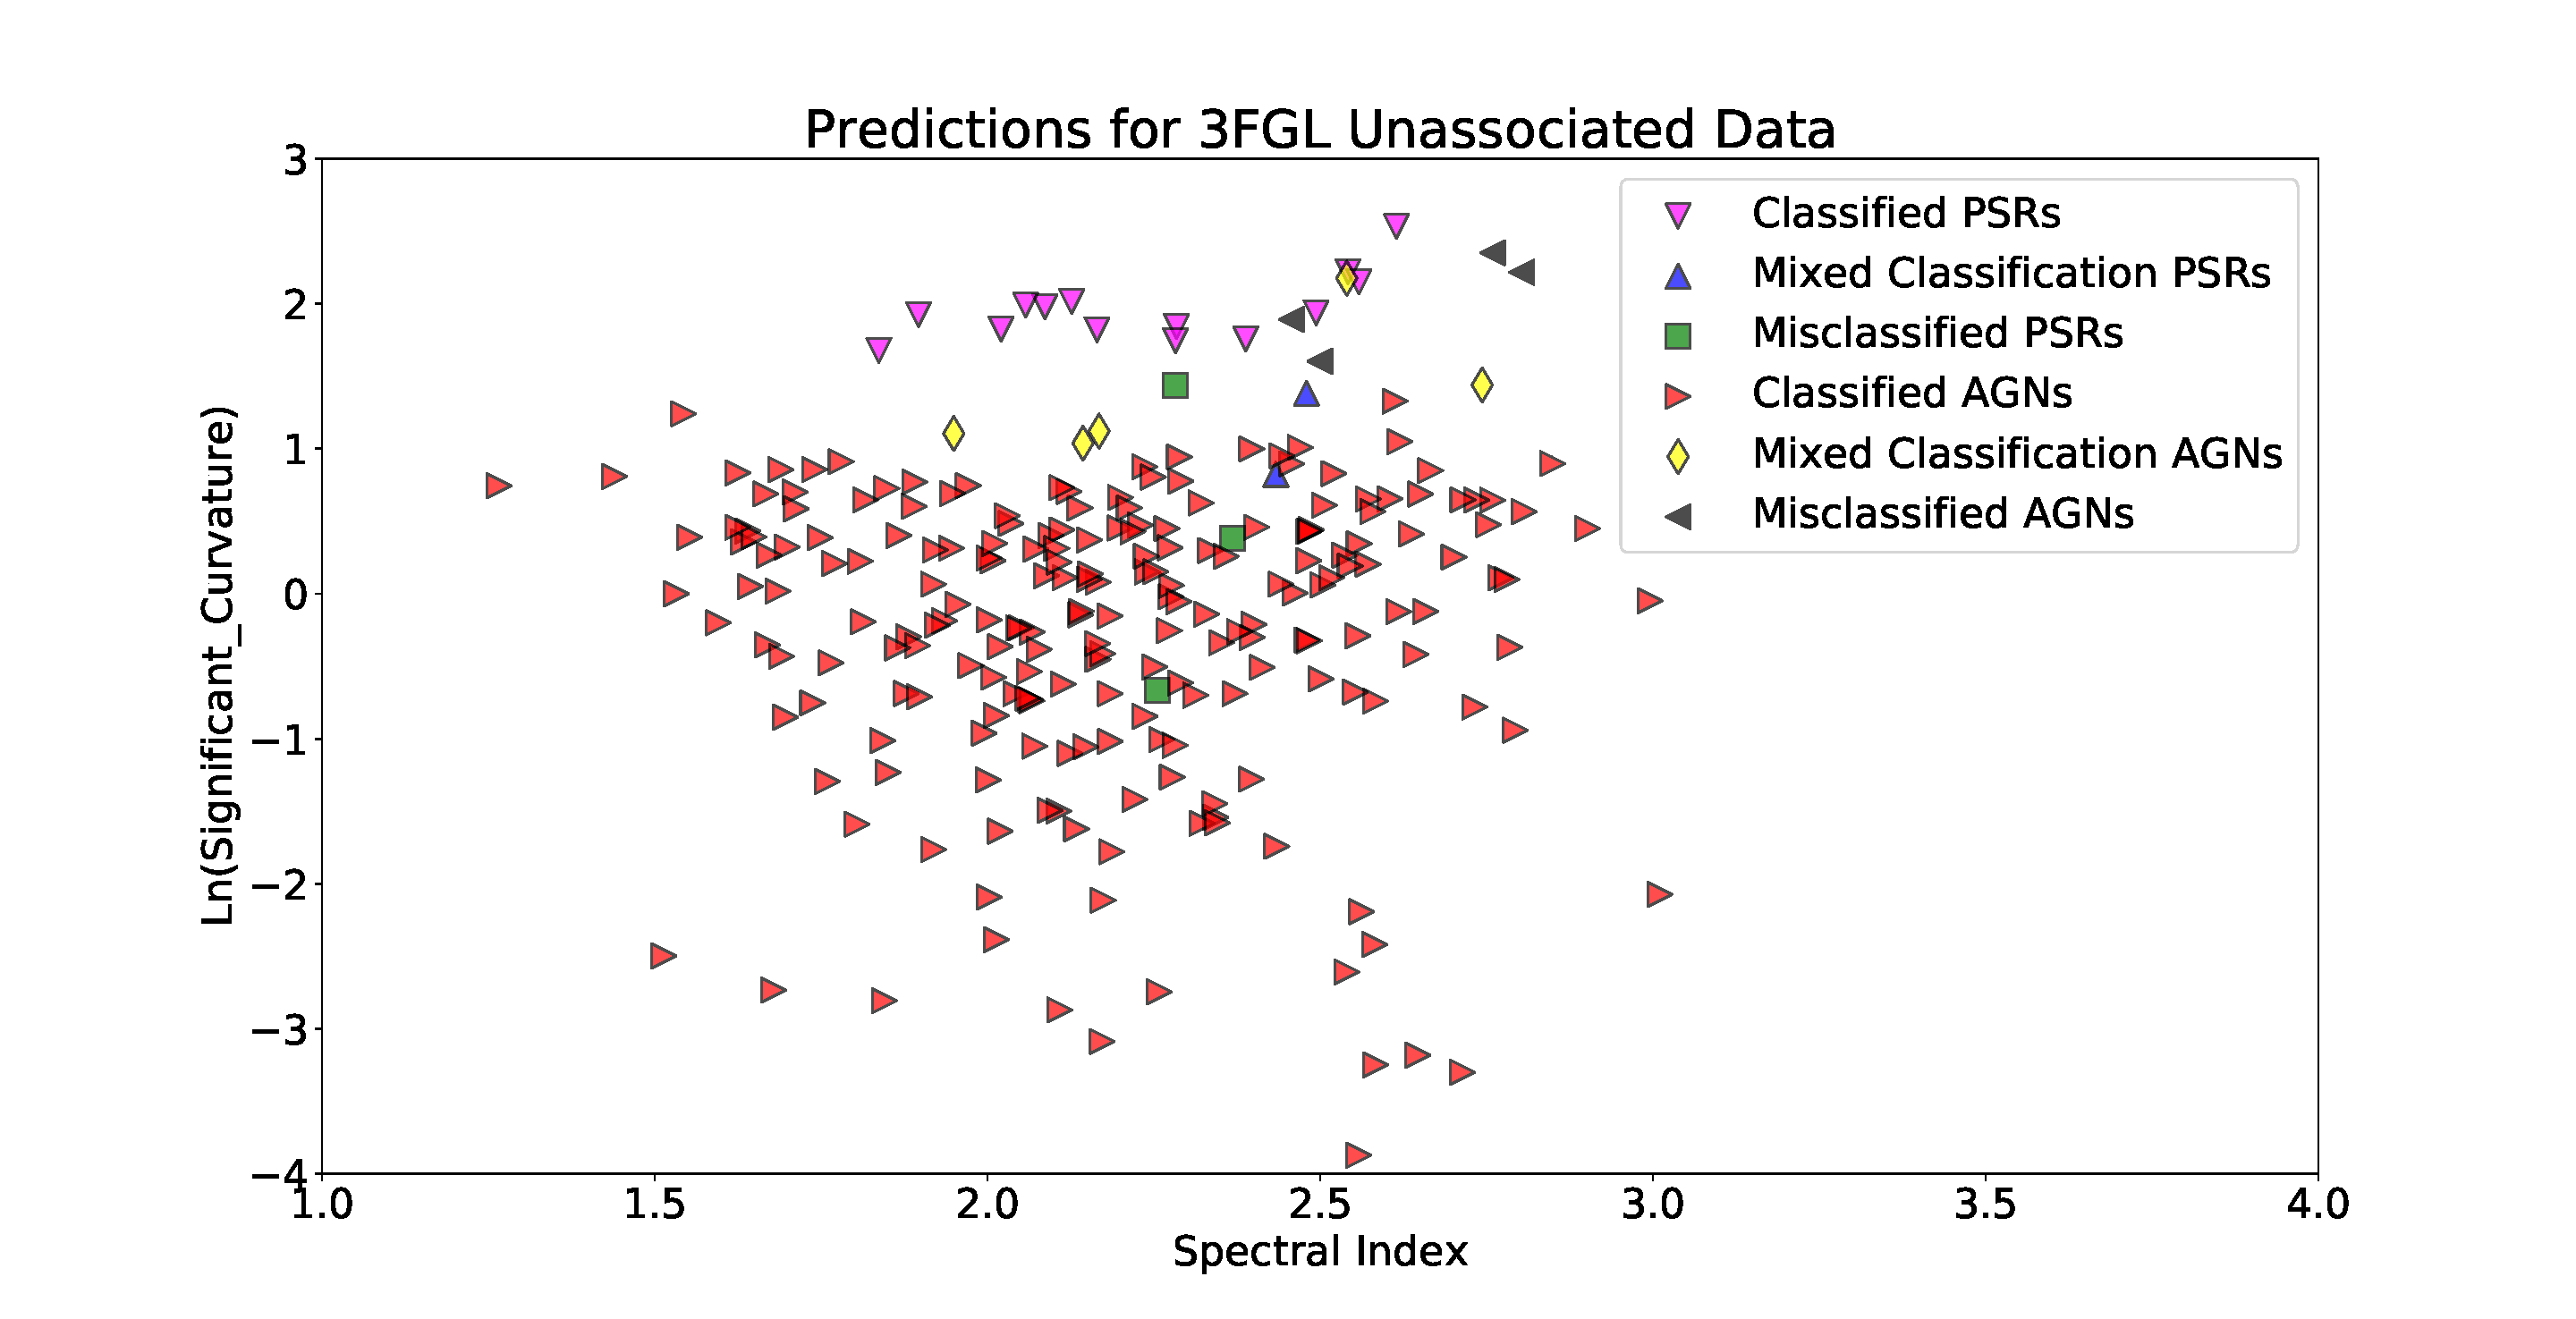
\includegraphics[width=\textwidth]{plots/plot_final.pdf}
%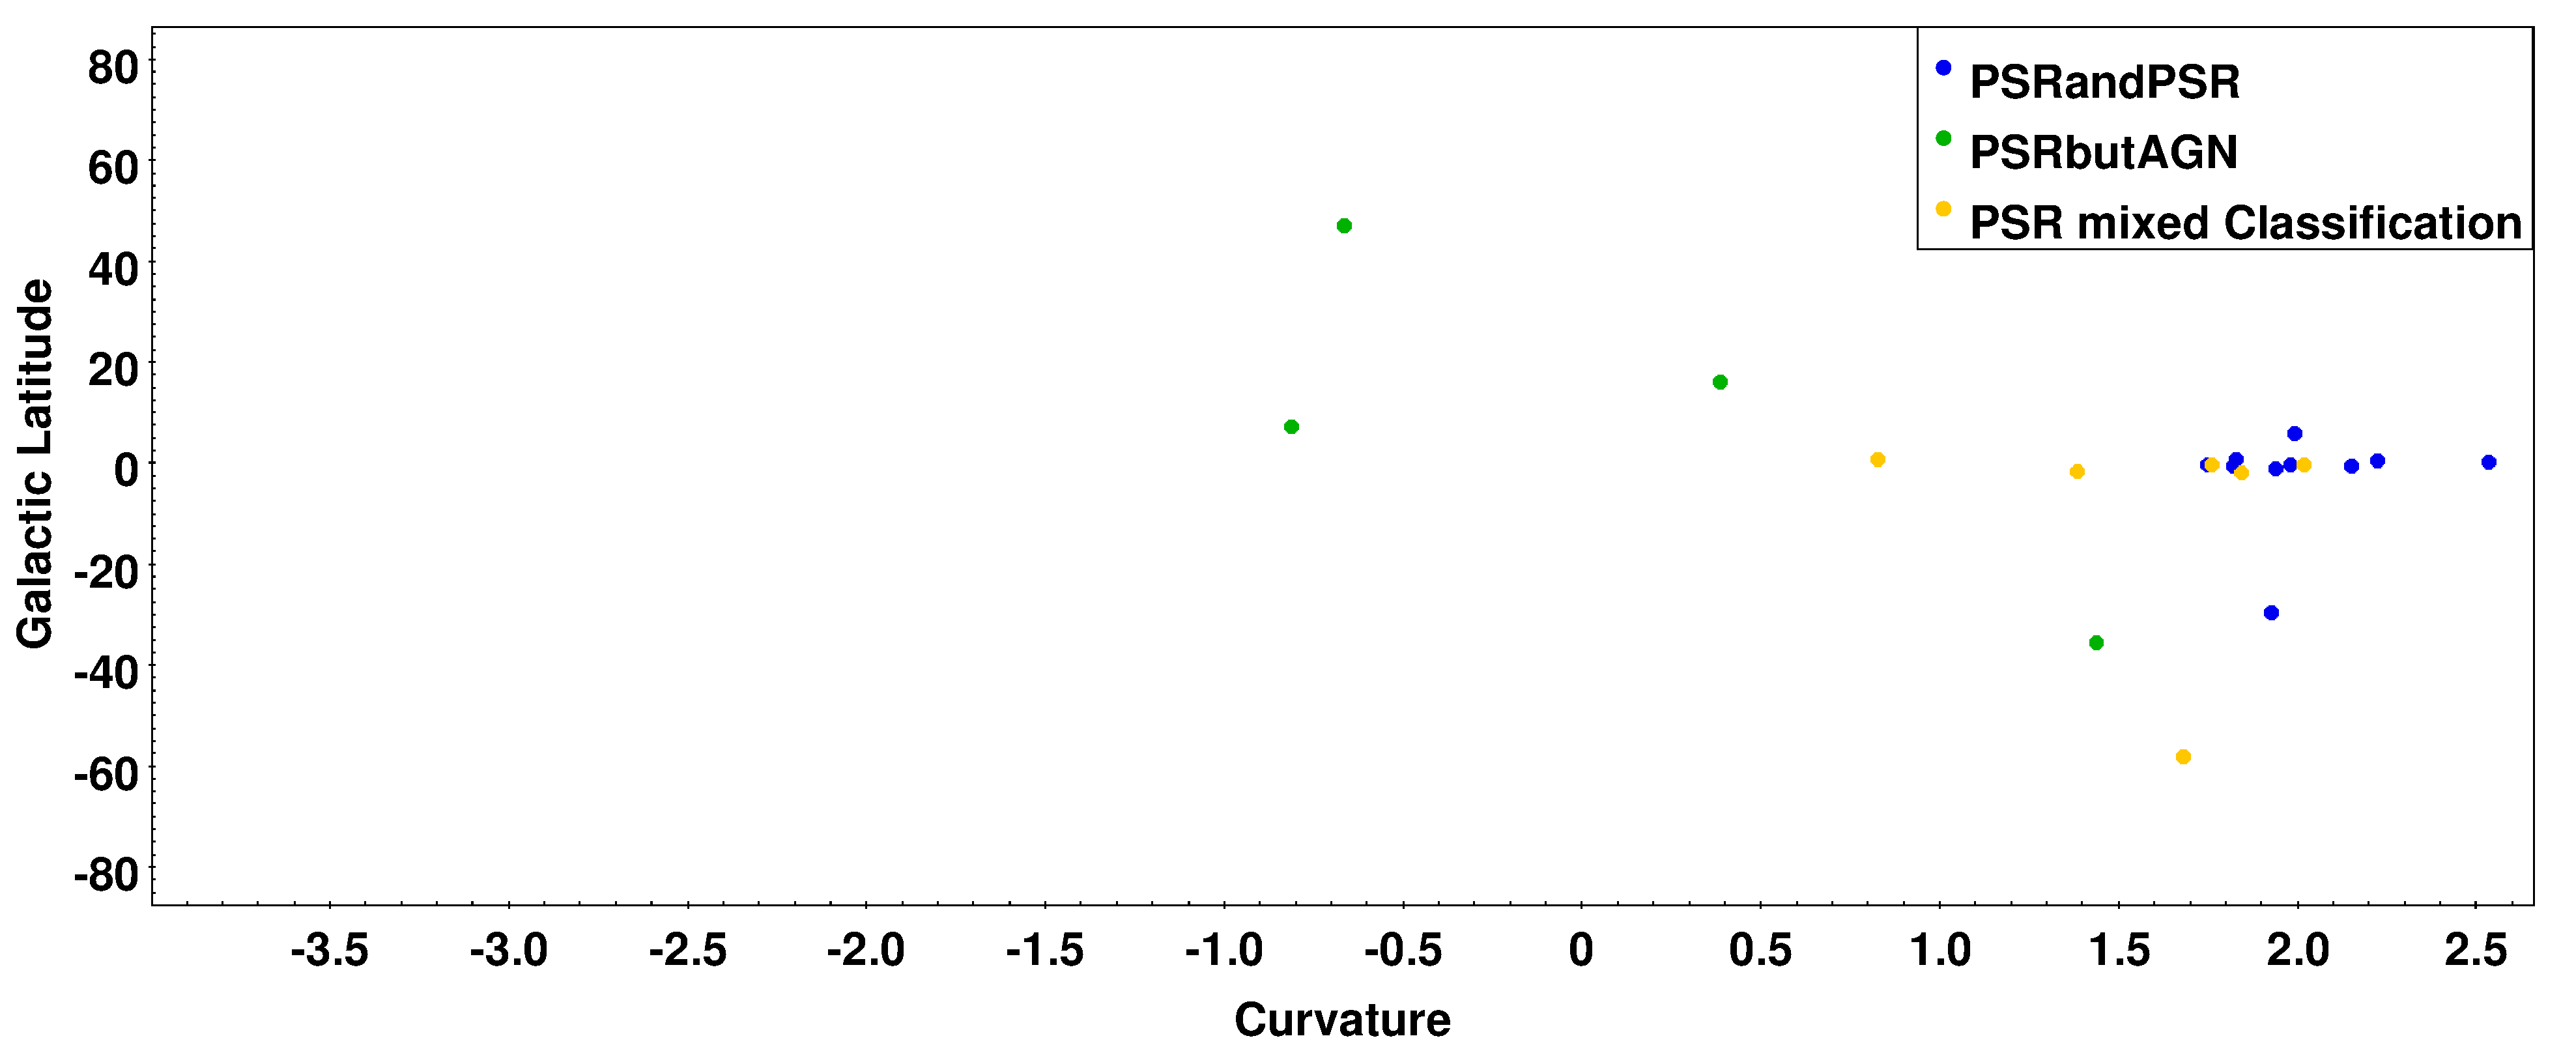
\includegraphics[width=\twopicsp\textwidth]{plots/PSR3.pdf}
\caption{Comparison of class prediction for unassociated 3FGL sources with classes in 4FGL. }
%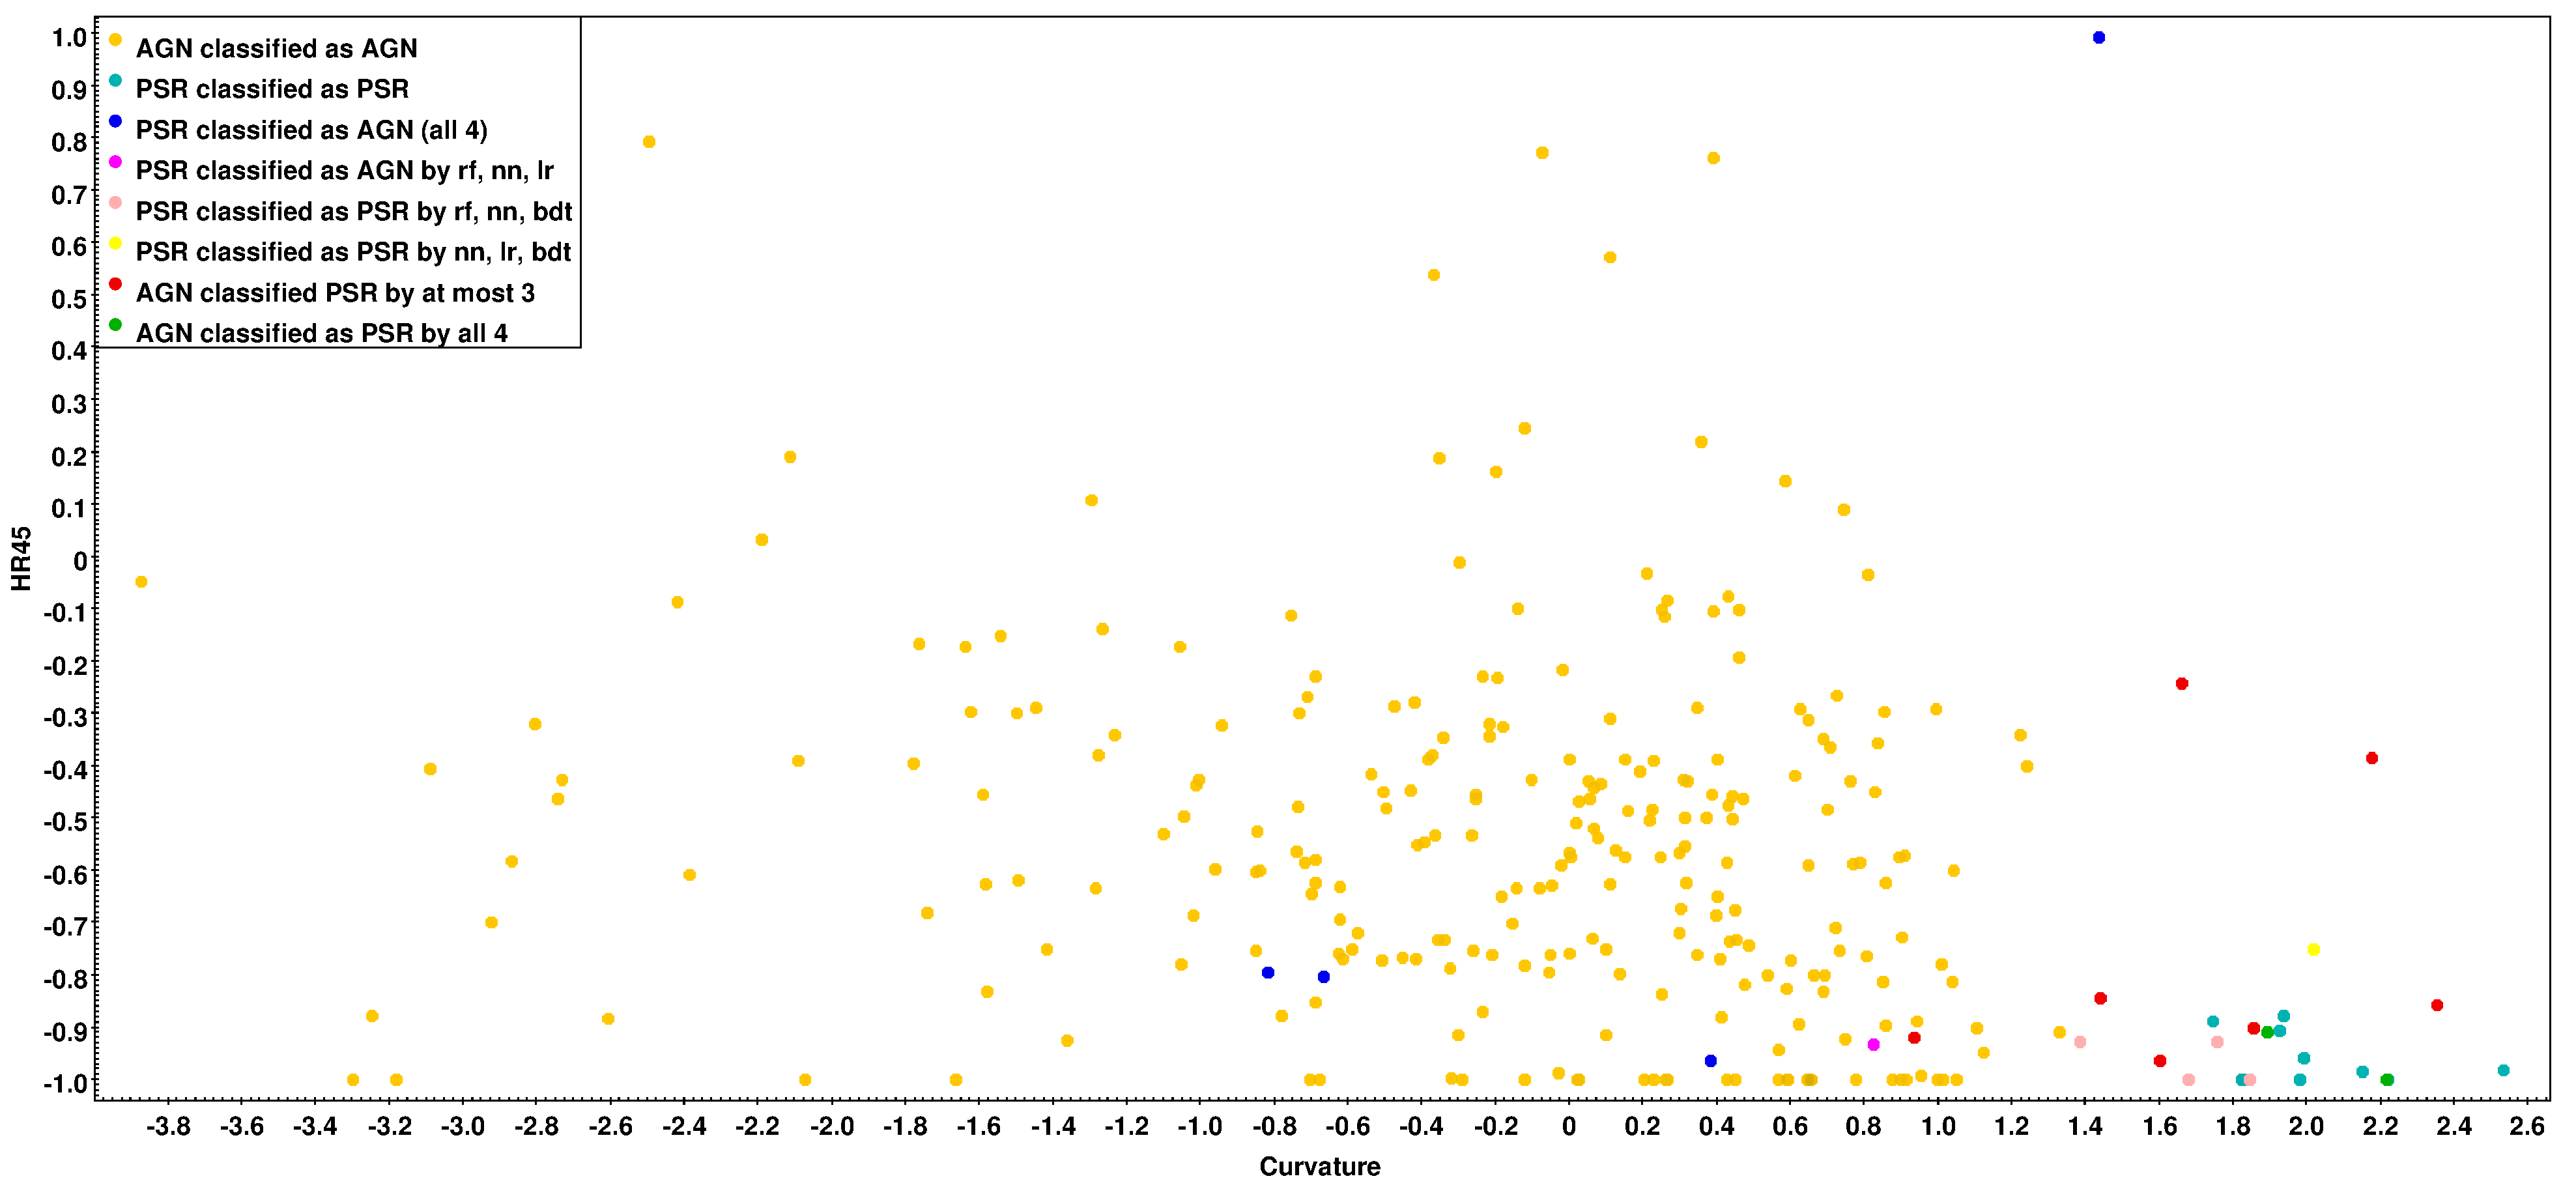
\includegraphics[width=\twopicsp\textwidth]{plots/final_catalog.pdf}
\label{fig:3FGL_vs_4FGL_classes}
\end{figure*}

As a result of the classification of 3FGL sources with the four ML algorithms,
we created probabilistic catalogs for unassociated and, separately, for associated 3FGL sources.
We have also subselected 242 unassociated 3FGL sources, which have PSR or AGN associations in 4FGL,
and saved them for convenience of comparison as a separate file, including characteristics from both 3FGL and 4FGL catalogs.
In the probabilistic catalogs we add columns with corresponding probabilities for each algorithm and each class,
i.e., provided that there are 4 algorithms and 2 classes, we add 8 columns.
Although the class probabilities for each algorithms should add up to one for every source, we still keep the columns for all classes for convenience.
Table \ref{tab:prob_cat} shows an example of the probabilistic catalog for a few unassociated 3FGL sources.
Notice that the first source is classified as a pulsar by BDT and as an AGN by RF, LR, and NN algorithms,
i.e., it will have a label ``classified either as PSRs or AGNs'' in Figure \ref{fig:3FGL_vs_4FGL_classes}.
The second and third sources are classified as AGNs by all four algorithms, i.e., they will have a label
``classified only as AGNs'',
while the last source is classified as a pulsar by all four algorithms, i.e., it will have a label
``classified only as PSRs''.
Overall, there are 97 unassociated sources classified as pulsars by all four algorithms, 729 sources classified as AGNs by all four algorithms, and 182 sources with mixed classifications.
Out of 97 sources classified as pulsars, 6 sources have counterparts in Parkes survey within 2 arc minutes.


\pgfplotstableread[col sep=comma]{data/catalogs/3FGL_unassoc_vs_4FGL_assoc.csv}\loadedtable
\begin{table}
\pgfplotstabletypeset[columns={Source_Name_3FGL,AGN_BDT,AGN_RF,AGN_LR,AGN_NN},
column type=l,
string type,
every head row/.style={before row={\toprule & \multicolumn{4}{c}{AGN Probability} \\},after row=\midrule,},
every last row/.style={after row=\vdots },
columns/Source_Name_3FGL/.style={column name=Source\_Name},
columns/AGN_BDT/.style={column name=BDT,numeric type,fixed,precision=3},
columns/AGN_NN/.style={column name=NN,numeric type,fixed,precision=3},
columns/AGN_RF/.style={column name=RF,numeric type,fixed,precision=3},
columns/AGN_LR/.style={column name=LR,numeric type,fixed,precision=3},
skip rows between index={4}{242}
]\loadedtable
\caption{\label{tab:prob_cat}
Example of the AGN classification probabilities for a few unassociated sources in the 3FGL catalog.}
\end{table}



\pgfplotstableread[col sep=comma]{data/catalogs/3fgl_unassoc_predictions_matches_with_Parkes(2015)_1.csv}\loadedtable
\begin{table}
\pgfplotstabletypeset[columns={3FGL,GLON,GLAT,Separation},
every head row/.style={before row={\toprule},after row=\midrule,},
every last row/.style={after row=\midrule },
columns/3FGL/.style={column name=Source\_Name,string type},
columns/GLON/.style={column name=GLON,numeric type,fixed,precision=1},
columns/GLAT/.style={column name=GLAT,numeric type,fixed,precision=1},
columns/Separation/.style={column name=Sep (arksec),numeric type,fixed,precision=1}
]\loadedtable
\caption{\label{tab:parkes}
Connection of unassociated 3FGL sources classified as PSRs with Parkes PSRs.}
\end{table}


\section{Prediction for unassociated source in the 4FGL catalog}
\lb{sec:4FGLprediction}

After having perused the 3FGL data we moved on to the 4FGL associated data. The 4FGL catalog has higher number of features, especially due to the difference in modeling when compared with the 3FGL. We selected 31 of these features and looked for the corelation between them. If Any feature was corelated or anti-corelated with a pearson index of $\pm$0.75 or higher with another, then only one of them was kept. This resulted in 17 features making it through in the end, which includes 10 of the original features we had used in the 3FGL catalog and and 2 more hardness ratios since 4FGL catalog has 2 more energy bands than 3FGL. The full corelation matrix with indices can be seen below.\\

\begin{figure*}[h]
\centering
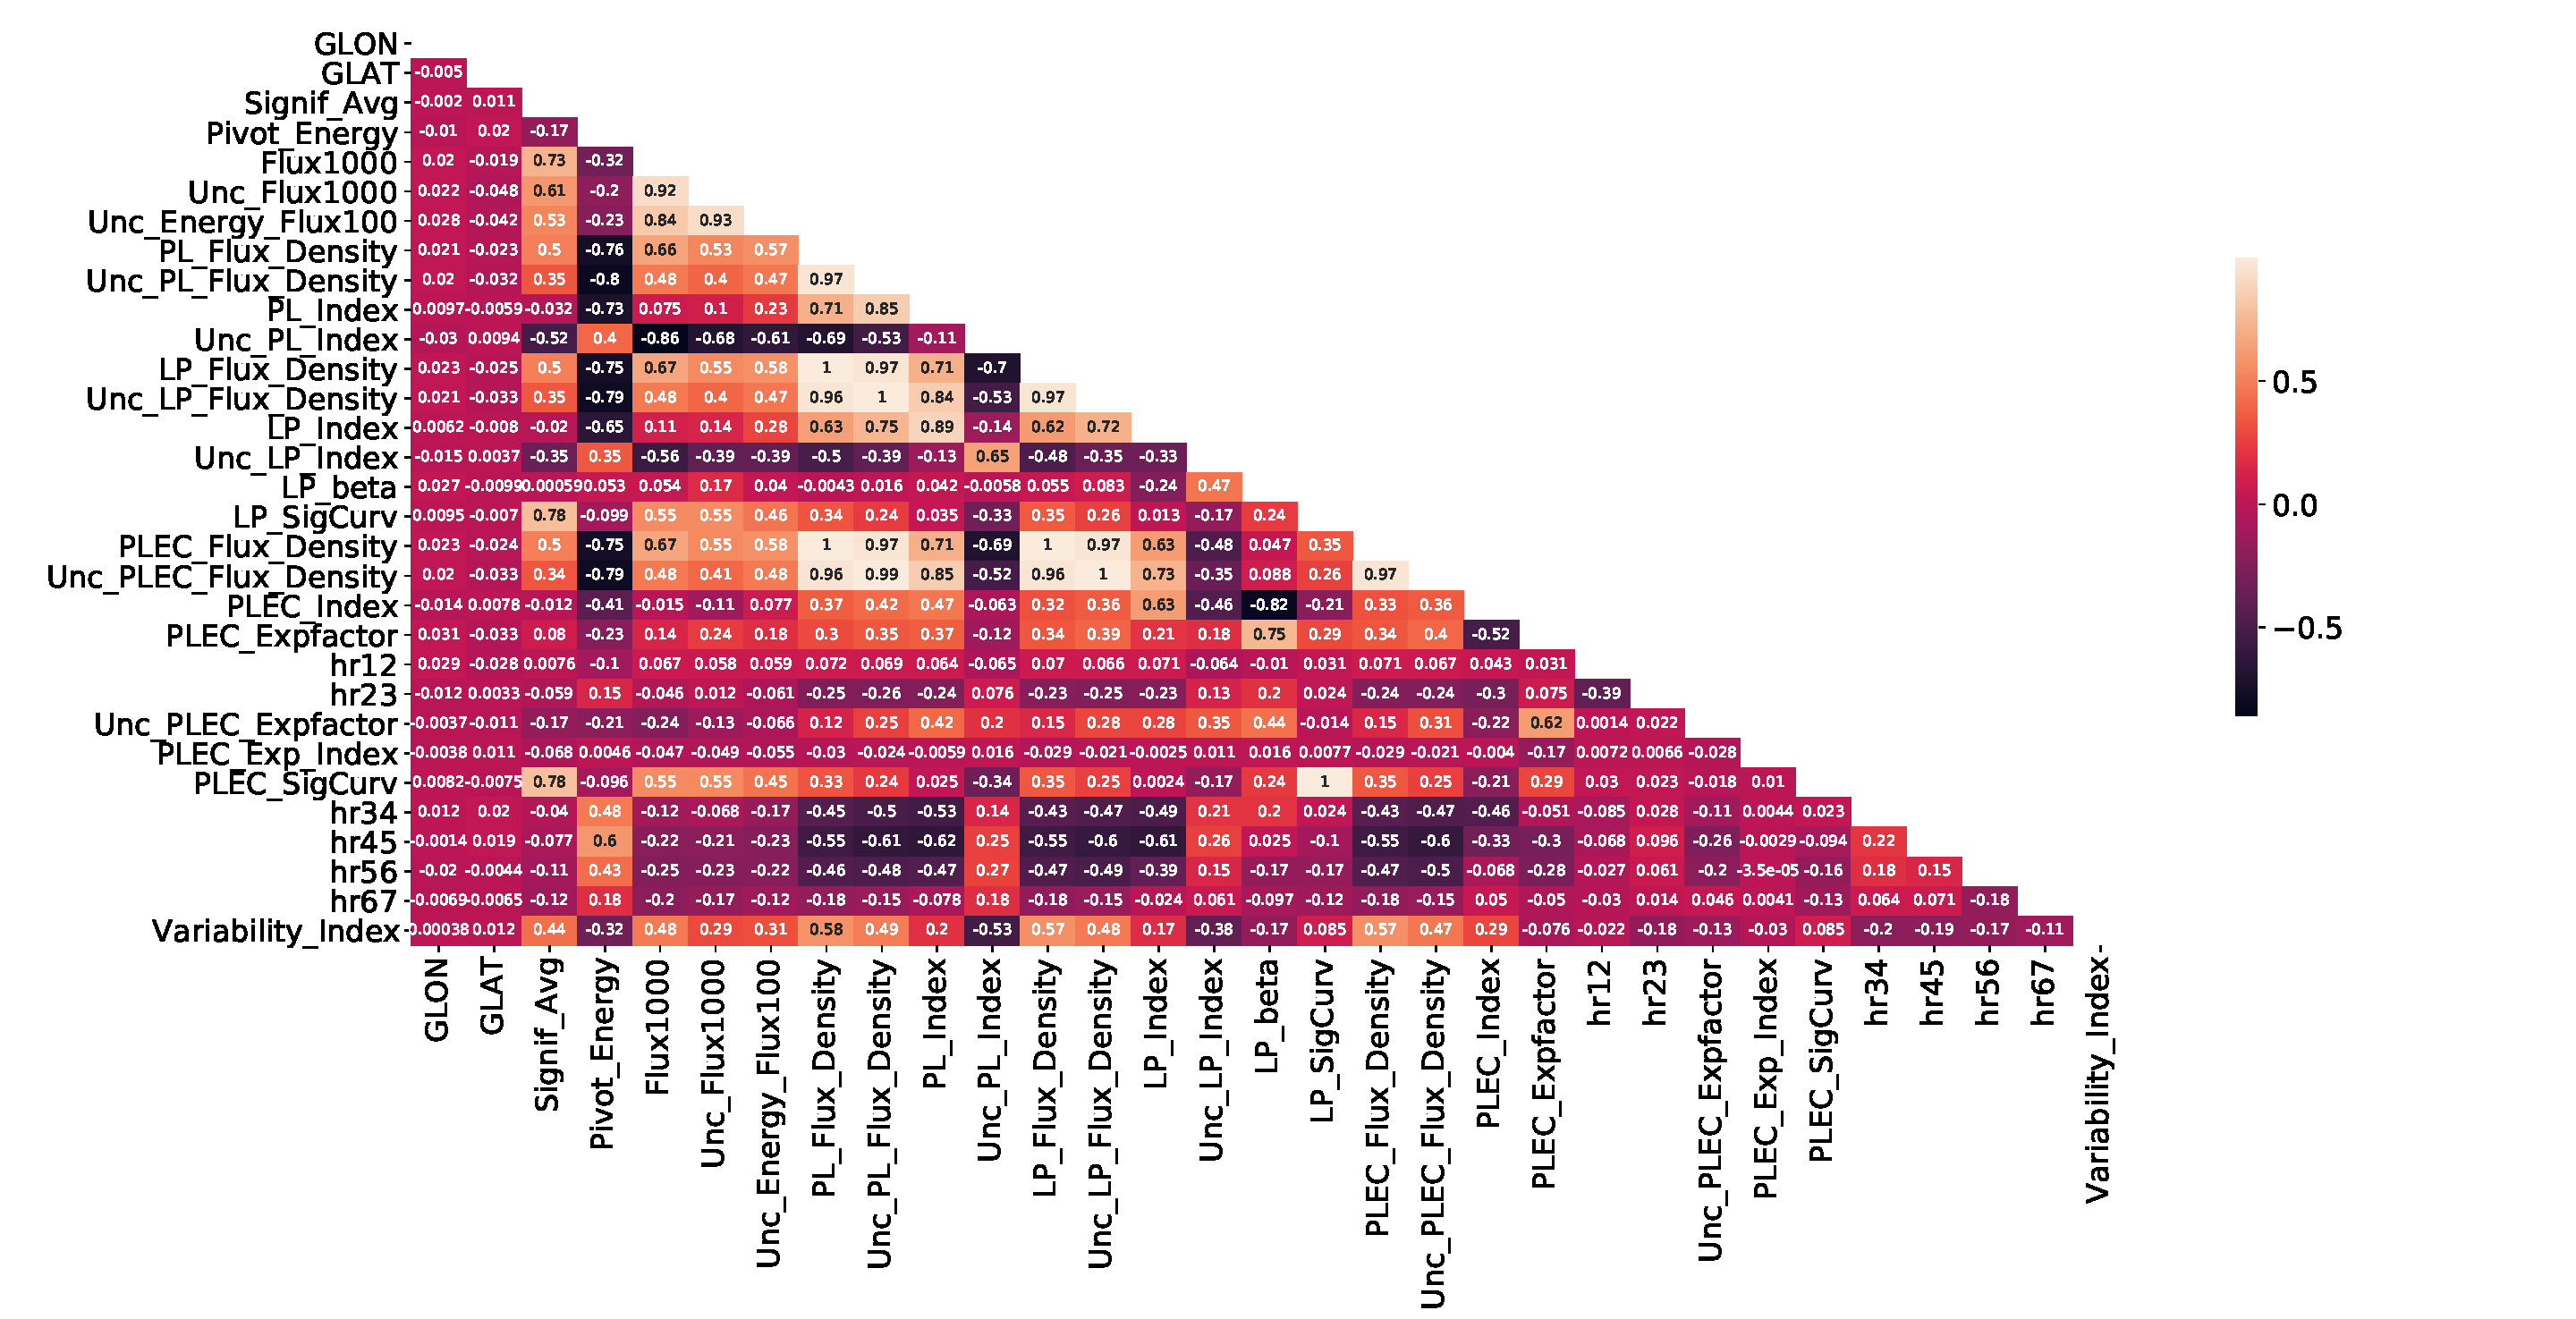
\includegraphics[width=\textwidth]{plots/correlation_4fgl_assoc.pdf}
%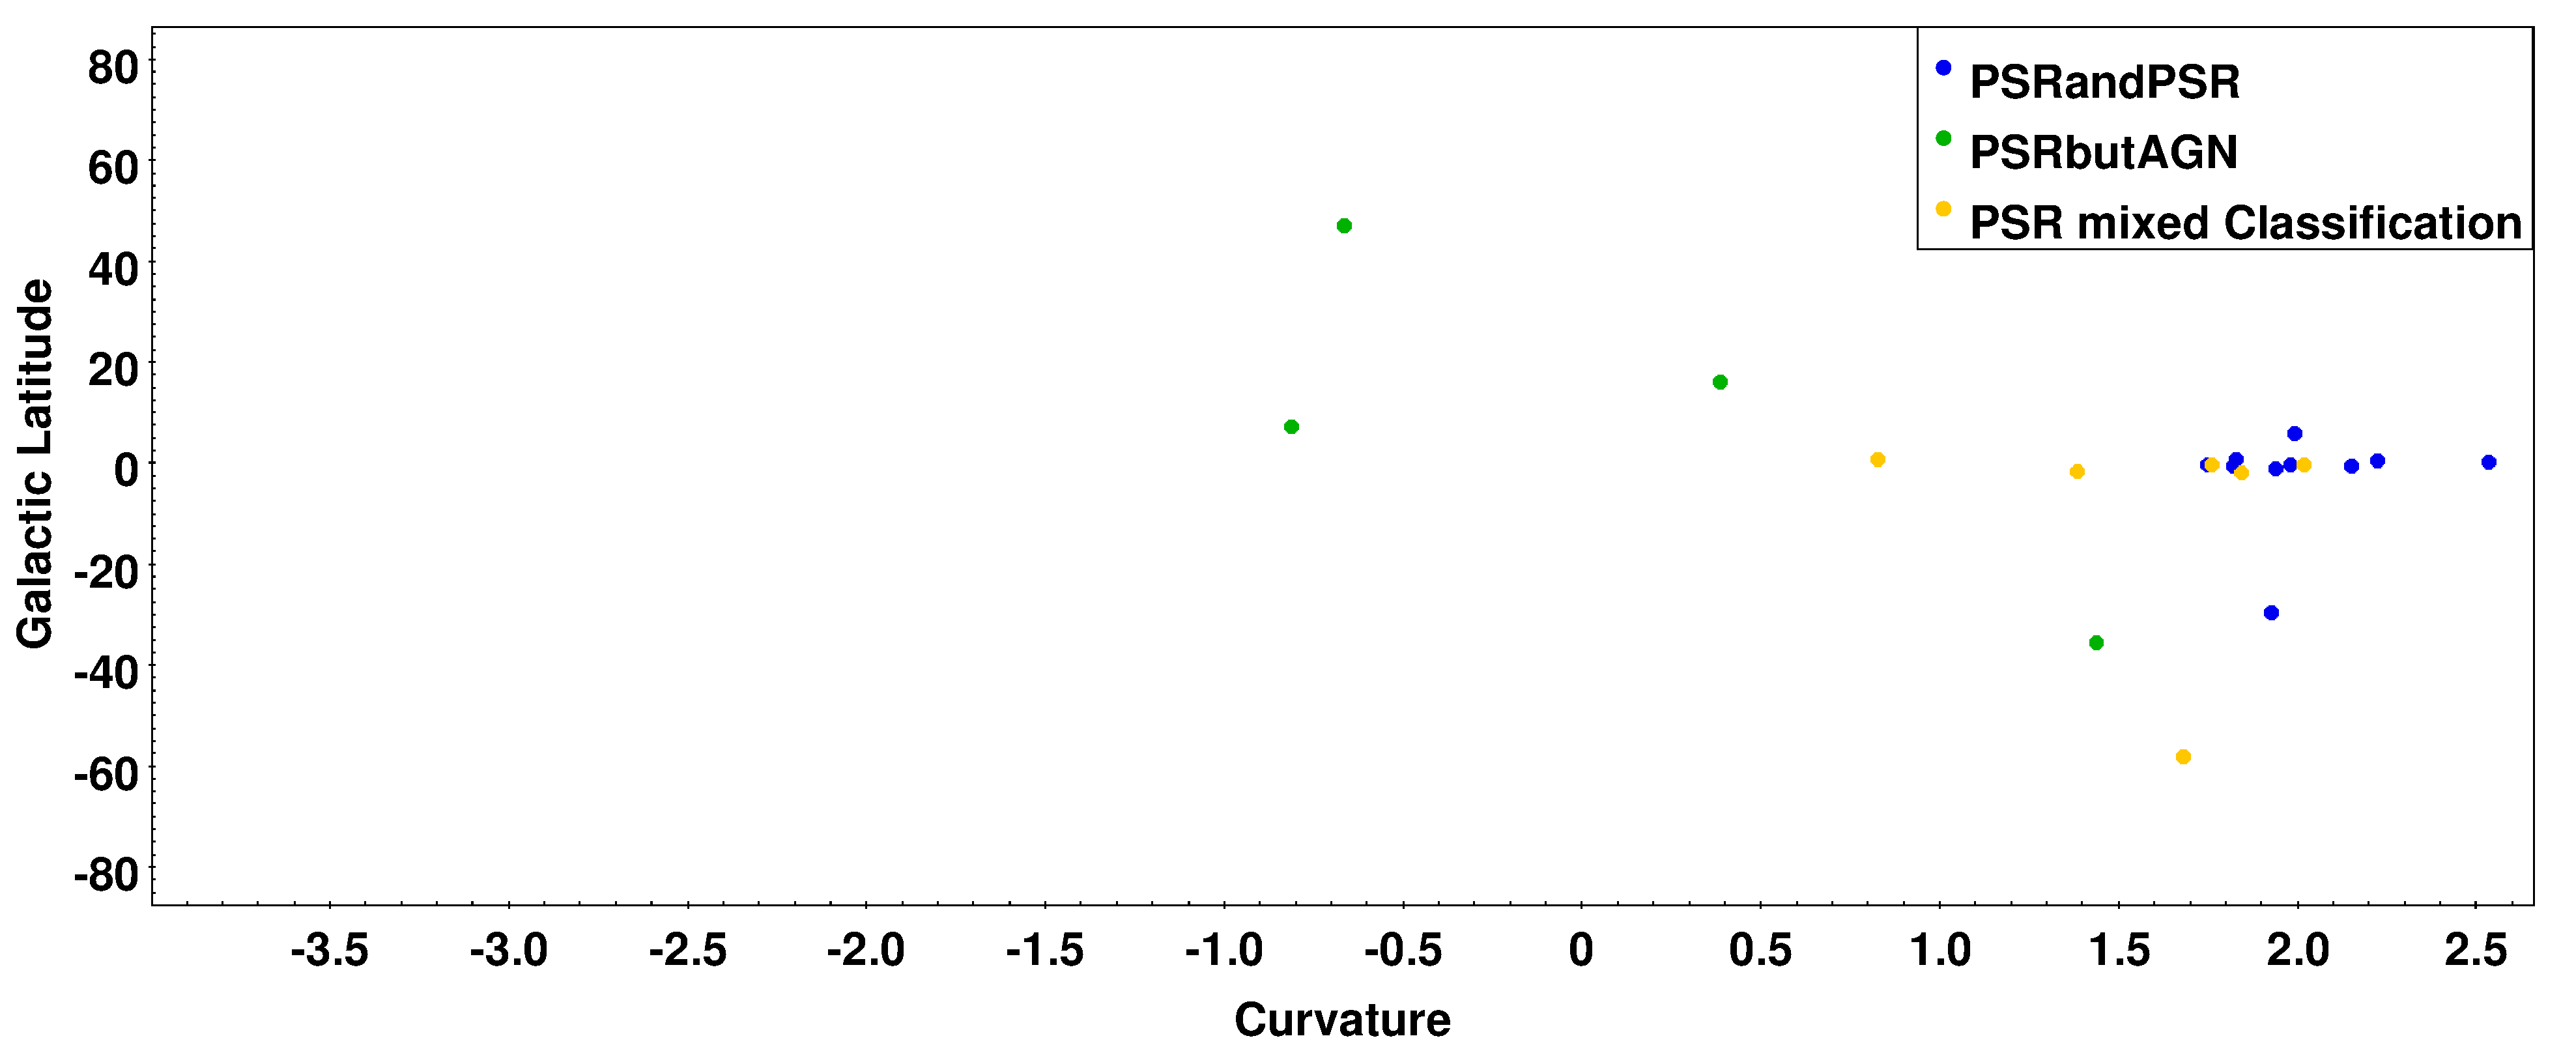
\includegraphics[width=\twopicsp\textwidth]{plots/PSR3.pdf}
\caption{Corelation matrix for 4FGL associated data }
%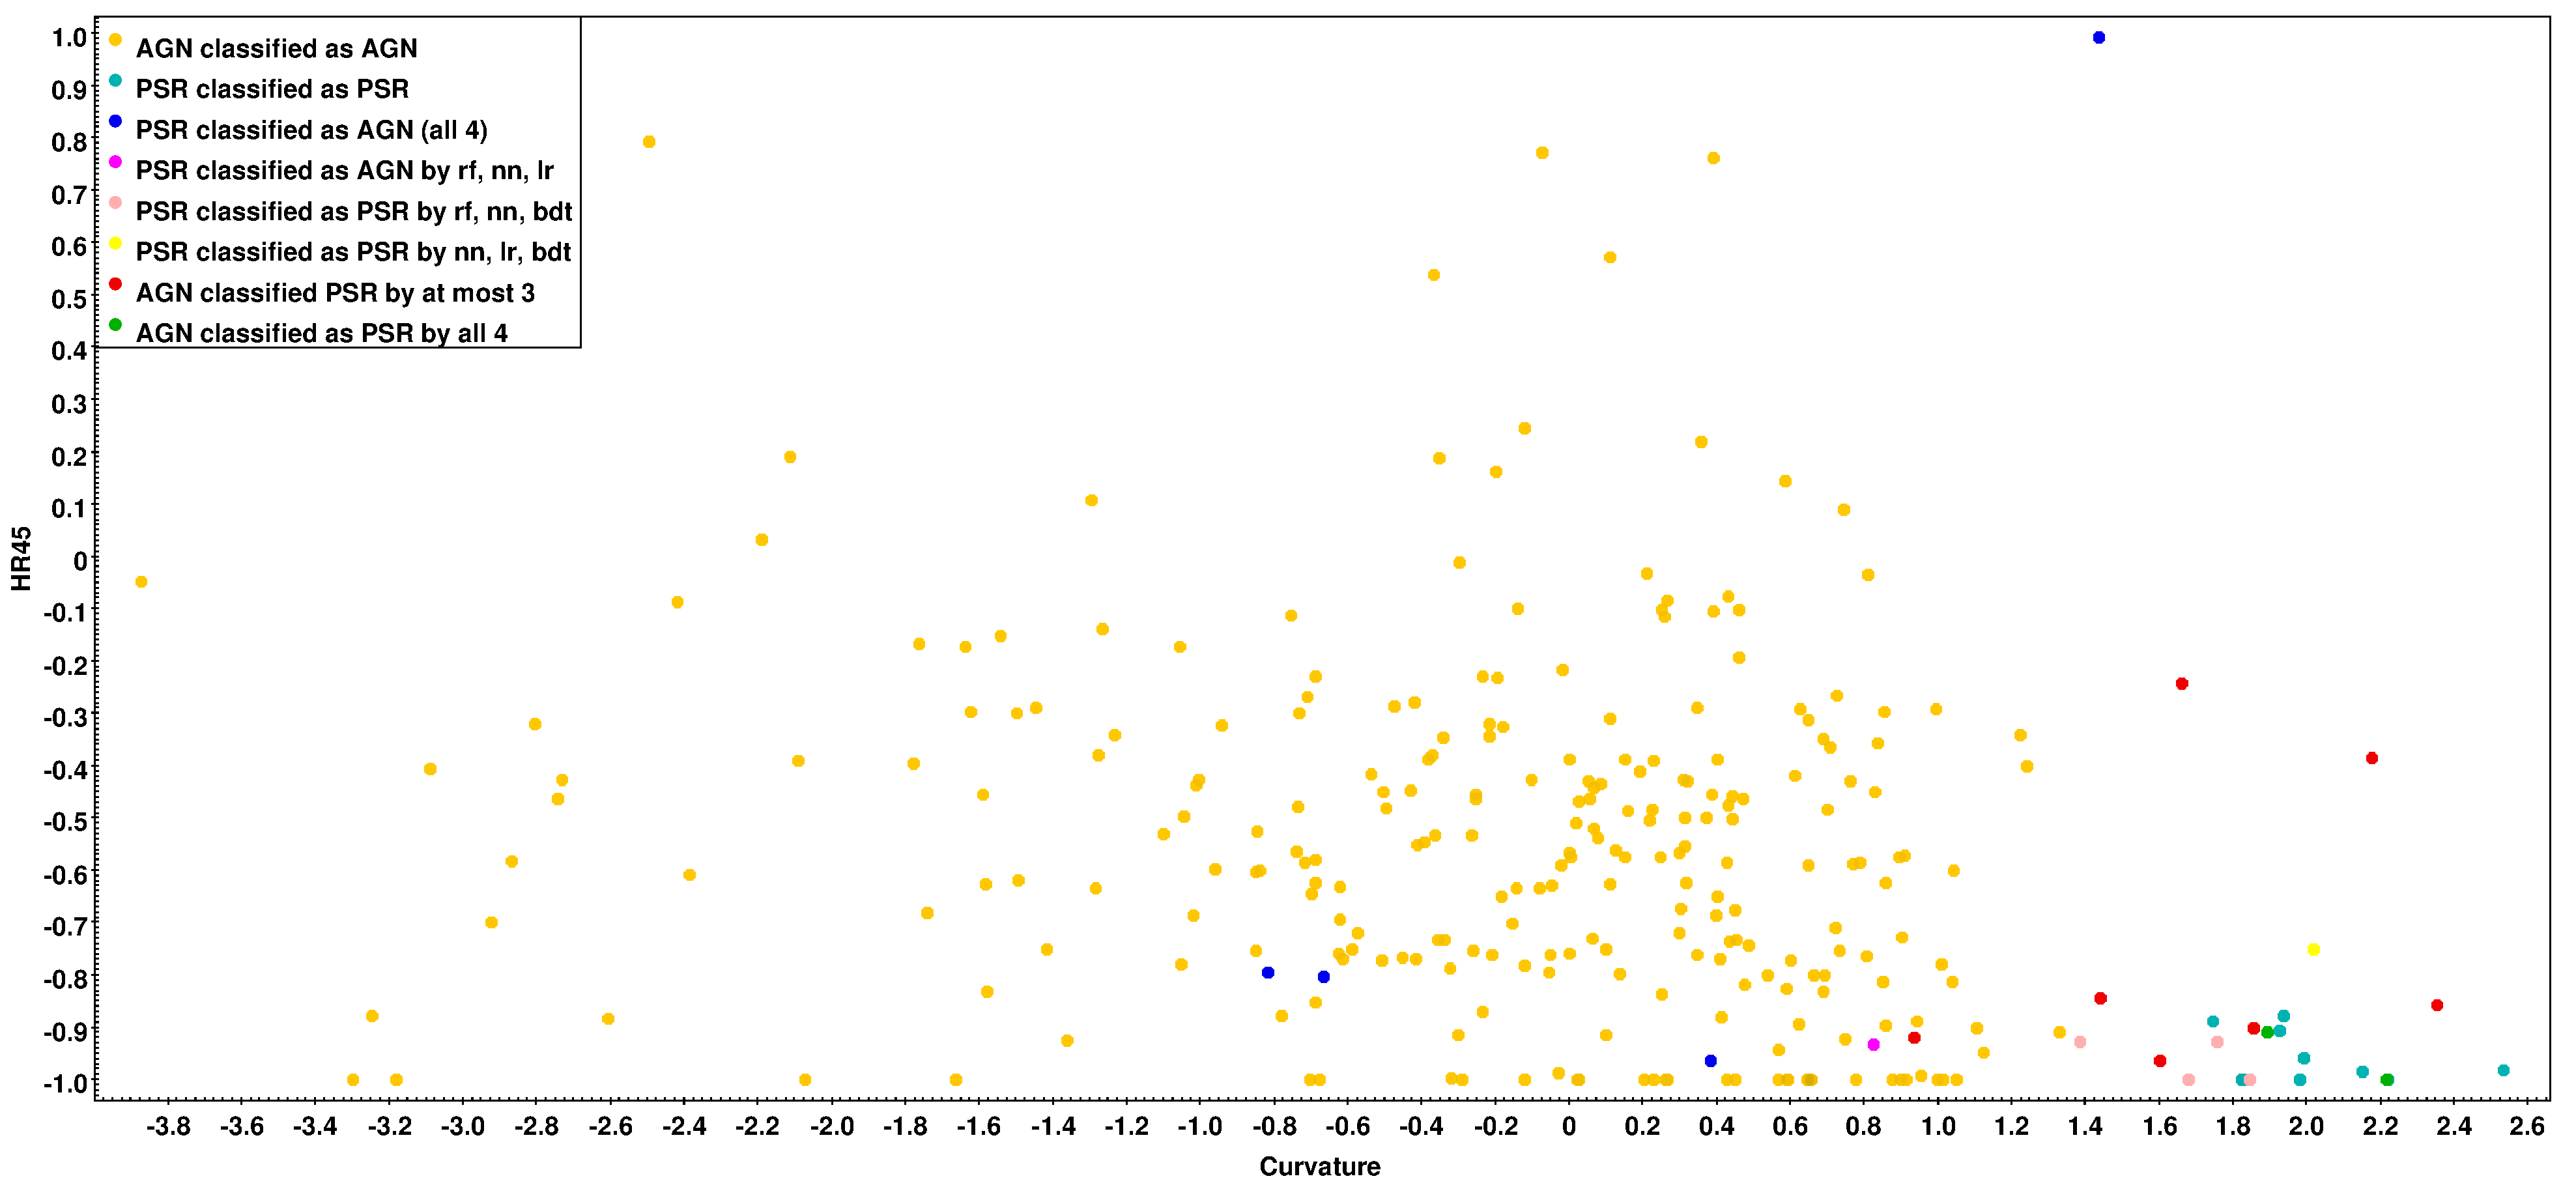
\includegraphics[width=\twopicsp\textwidth]{plots/final_catalog.pdf}
\label{fig:corr_mat}
\end{figure*}


In this section, we chose not to do another preliminary analysis of the algorithms. Therefore we used the same chosen algorithms as before, except with the neural network where we increased the number of neurons to 17 (same as the number of features). However, due to the number of features being higher, we hypothesized that the Neural Network should under-perform as compared to before.
\begin{table}[!h]

\resizebox{0.45\textwidth}{!}{
    \tiny
 %  \centering
    \renewcommand{\tabcolsep}{0.3mm}
\renewcommand{\arraystretch}{1.5}

    \begin{tabular}{|c|c|c|}
    \hline
    Algorithm&Parameters & Testing Accuracy \\
    \hline
    RF& 50 trees, max depth 6  &98.27\\
    \hline
    NN & 300, 17 Neurons, Adam & 98.08\\
    \hline %\midrule   -> aakash do you mean this?
    BDT & 100 trees, max depth 2    &   98.23\\
%    \hline %\midrule   -> aakash do you mean this?
%    BDT & 200 trees, max depth 2    &   95.8  \\
    \hline
    LR & LBFGS solver, 200 iterations & 98.08\\
    \hline
     
    \end{tabular}}
    \vspace{0.2cm}
    \caption{Accuracy of the 4 selected algorithms on 4FG associated data.}
    \label{tab:selected_algs2}
\end{table}

As can be seen in the table above, all algorithms except the Neural Network perform better, reaching more than 98\% accuracy. 


